	\begin{figure}[h]
	\centering
		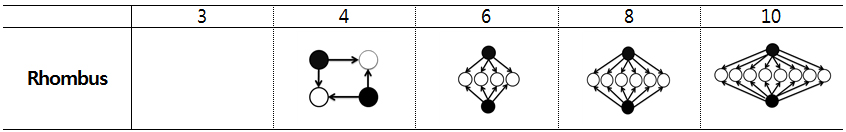
\includegraphics[height=50pt]{Topologies_Rhombus}
		\caption{Bayesian Network Topologies : Rhombus}
	\end{figure}	

	% Rhombus는 두 개의 node가 여러 개의 자식 node를 함께 가진 형태이다.
	Rhombus is in the form of two of the node is attached multiple of the child node together.

\begin{figure}[!bhp]
	\centering
		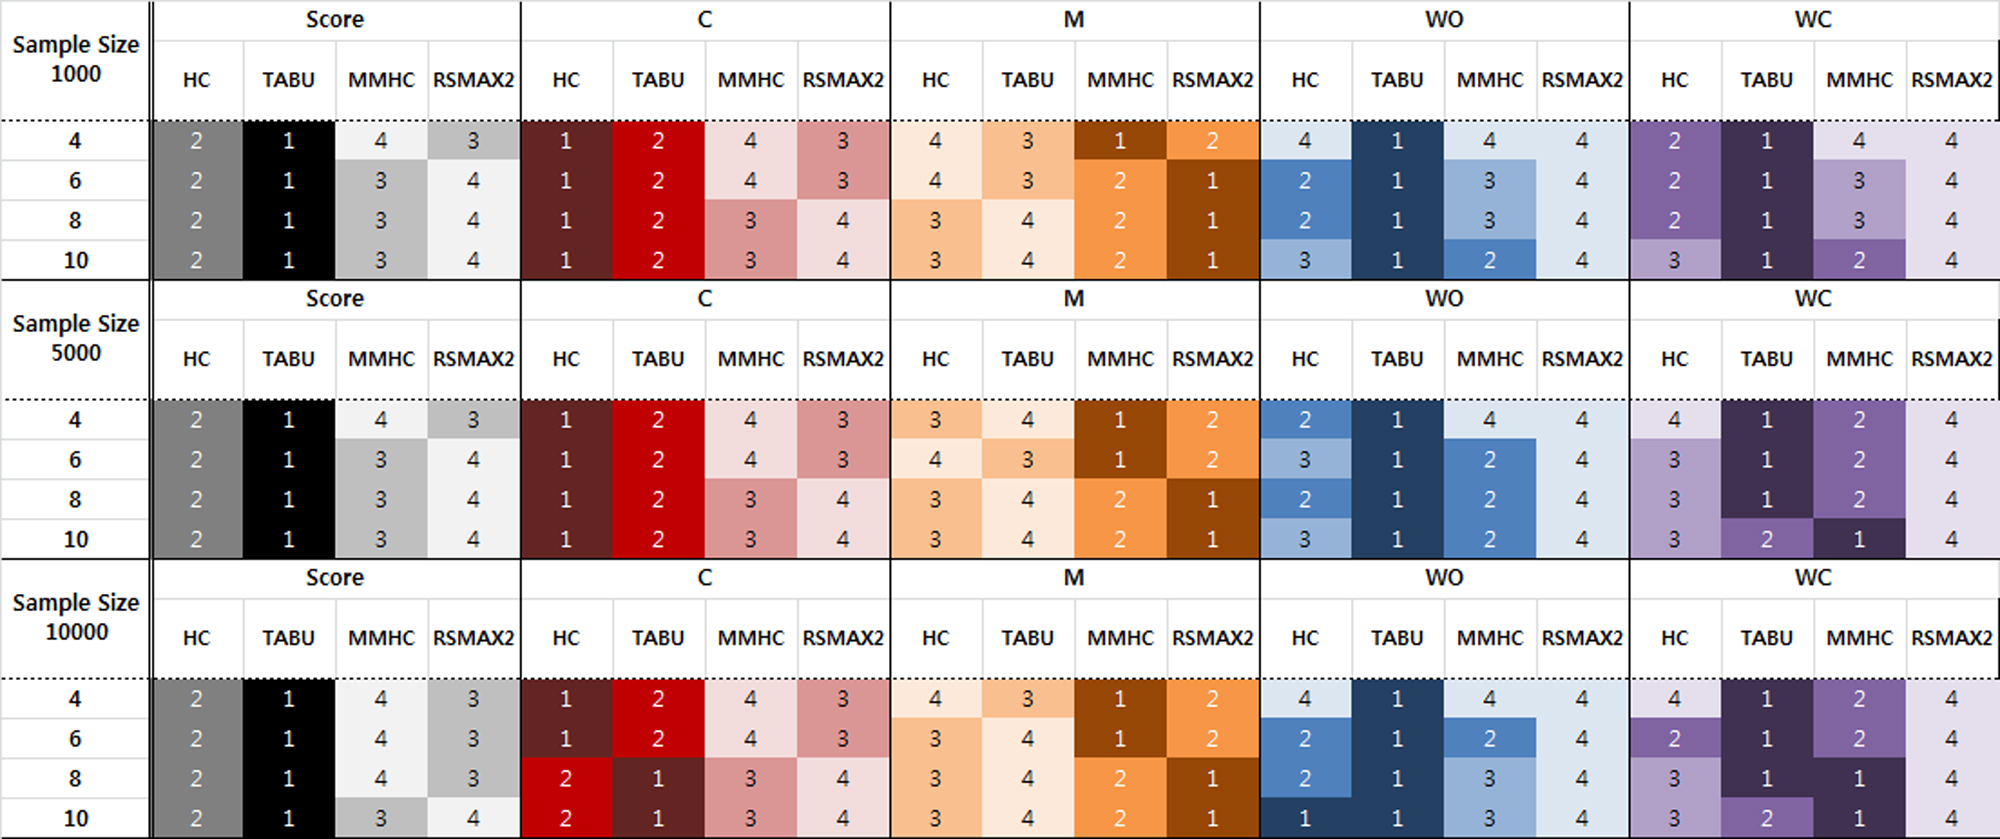
\includegraphics[height=170pt]{Result_Rhombus}
		\caption{Summary for Comparison via Rhombus}
	\end{figure}	

% Score, C 기준으로 비교했을 때 각각 TABU search, Hill-climbing이 좋은 성능을 나타냈다.
Score, when compared on the basis of the C, TABU search, the Hill-climbing showed good performance, respectively.

% 하지만 WO, WC도 많은 것으로 나타났다.
However, WO, WC was also found many things.

% WO, WC가 적은 것을 기준으로 보았을 때 RSMAX2가 유리한 것으로 나타났다. 오히려 MMHC는 WC가 많이 나타났다.
WO, RSMAX2 when viewed relative to that WC is small it was found to be advantageous. Rather MMHC became many WC.

% 다만 sample size가 커짐에 따라 모든 알고리즘의 성능이 전반적으로 개선되는 모습이 나타났다.
However as the sample size increases, how the performance of all algorithms is overall improvement was revealed.
	
	\begin{figure}[p]
	\centering
		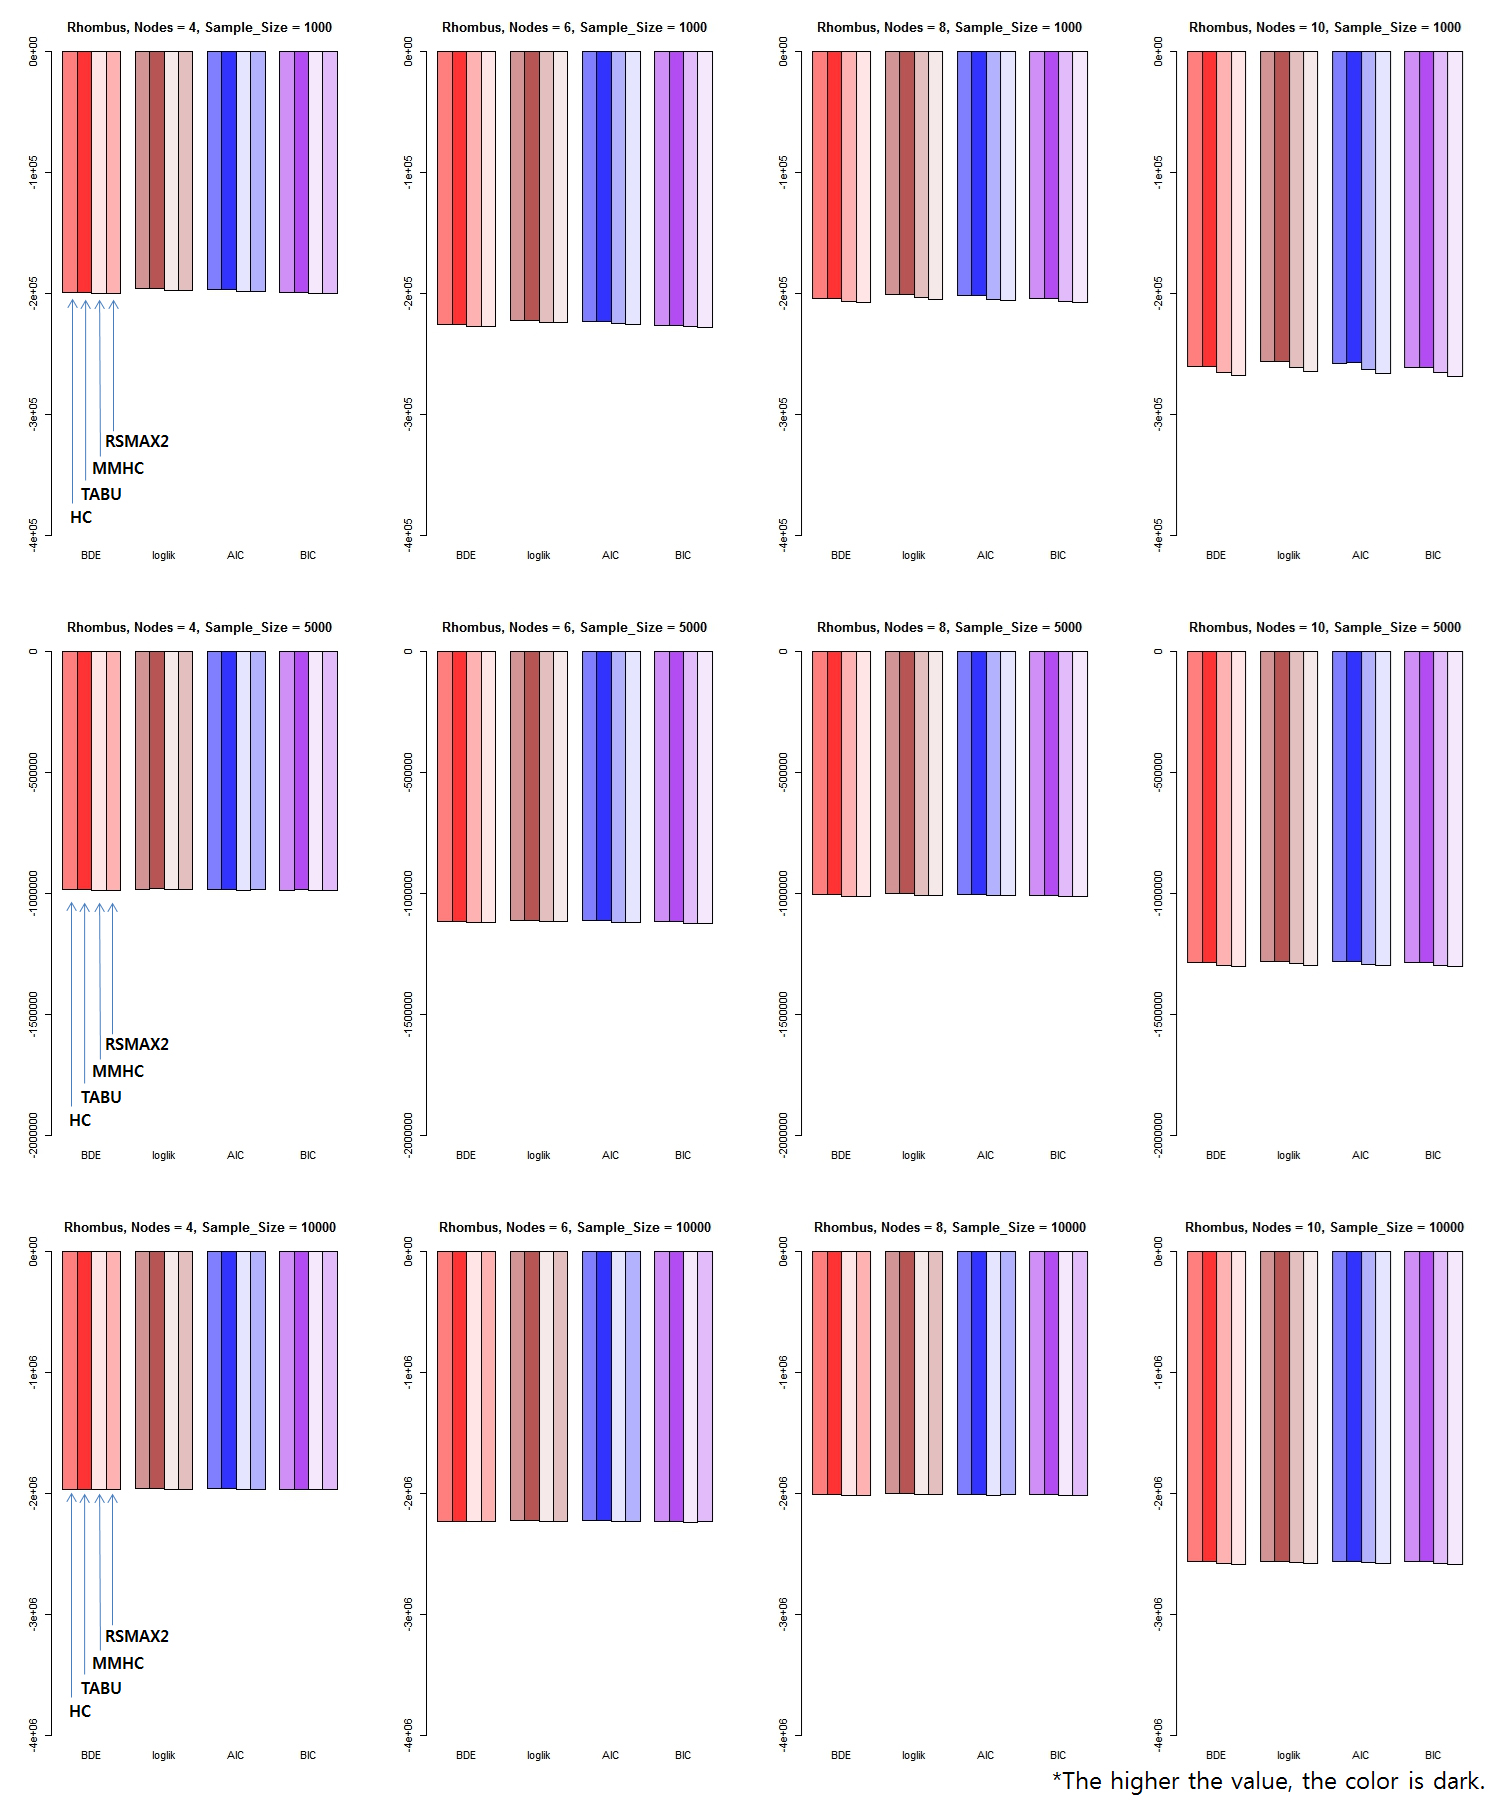
\includegraphics[height=500pt]{06_Rhombus_Score}
		\caption{Comparison of scores via Rhombus}
	\end{figure}	

	\begin{figure}[p]
	\centering
		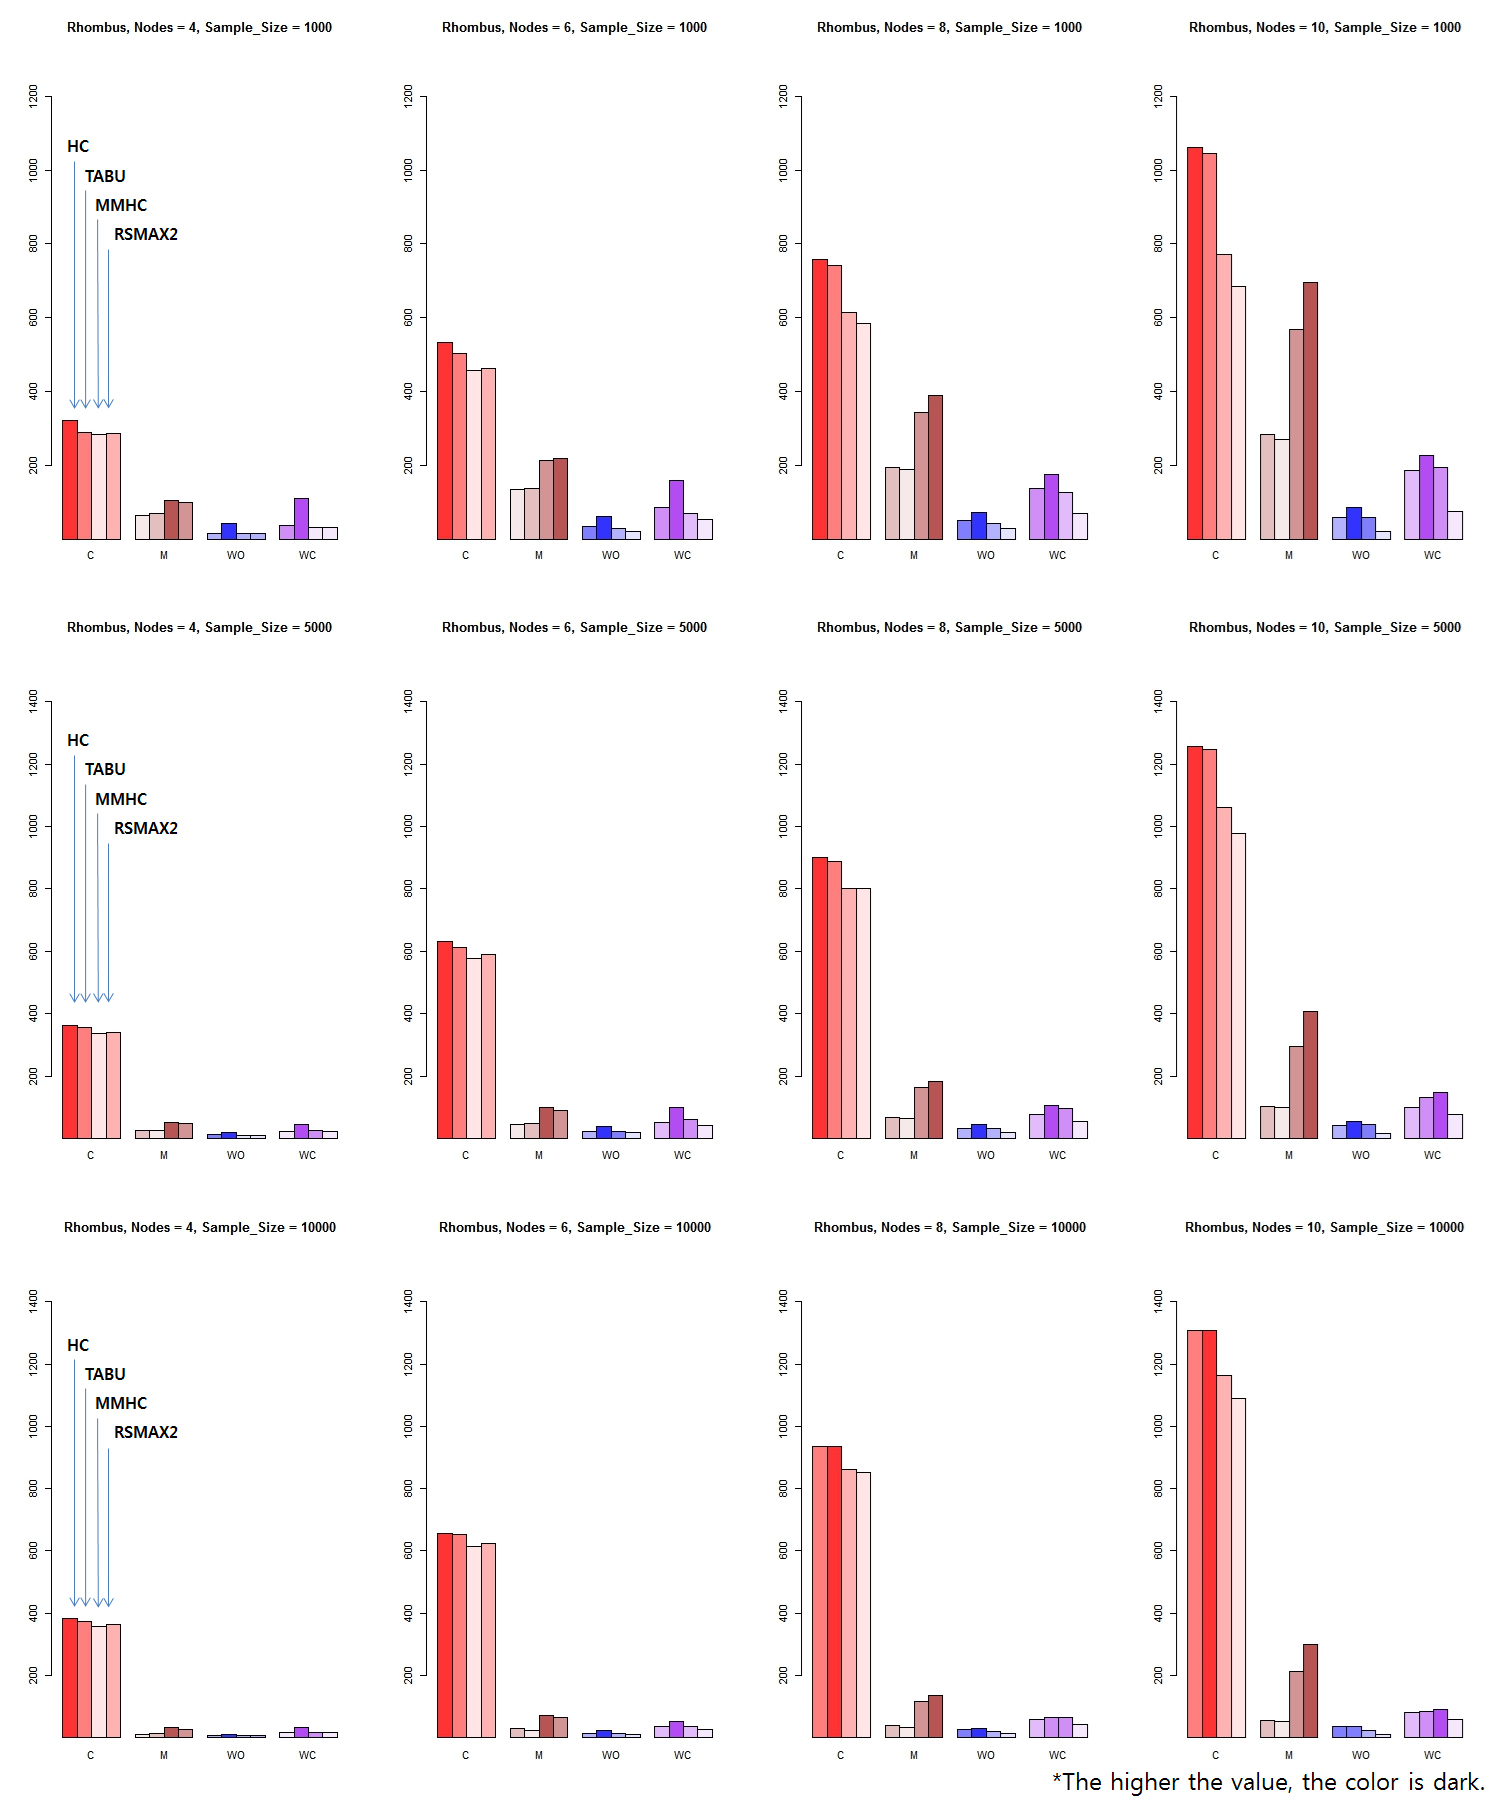
\includegraphics[height=500pt]{06_Rhombus_Arcs}
		\caption{Comparison of correct arcs via Rhombus}
	\end{figure}	
